\documentclass[border=4pt]{standalone}
% Shared typography and colours for the standalone figures.
\usepackage{unicode-math}
\setmainfont{TeX Gyre Termes}
\setmathfont{TeX Gyre Termes Math}
\usepackage{tikz}
\usetikzlibrary{arrows.meta,positioning,calc,decorations.pathreplacing}
\usepackage{pgfplots}
\pgfplotsset{compat=1.18}

% One colour per element or subsystem. Record the mapping in
% the working repository conventions and use it identically in every figure.
\definecolor{elemA}{HTML}{1F5FA8}
\definecolor{elemB}{HTML}{B8461B}
\definecolor{elemC}{HTML}{2E7D32}
\definecolor{elemD}{HTML}{6A4C93}
\definecolor{frameline}{HTML}{555555}

\begin{document}
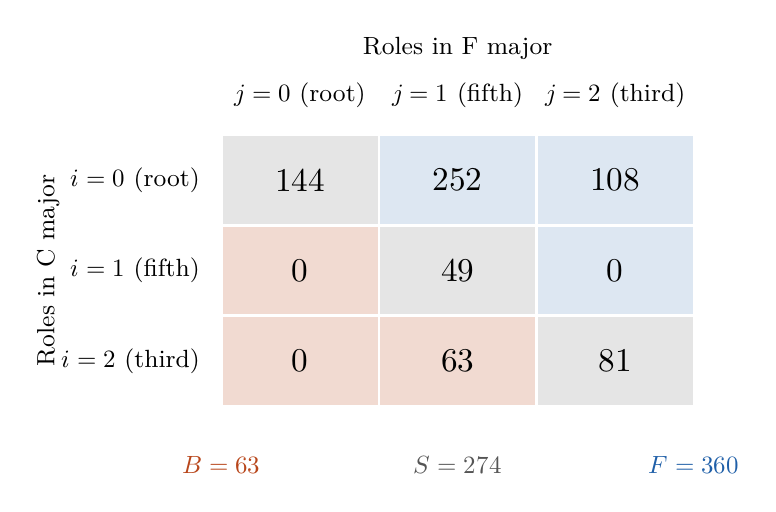
\begin{tikzpicture}[font=\small]
\foreach \i in {0,1,2} {
 \foreach \j in {0,1,2} {
  \ifnum\i<\j \def\shade{elemA!15}\else\ifnum\i>\j \def\shade{elemB!20}\else\def\shade{frameline!15}\fi\fi
  \filldraw[fill=\shade,draw=white,line width=1pt] (2*\j,-1.15*\i) rectangle +(2,-1.15);
 }
}
\foreach \x/\y/\v in {1/-0.575/144,3/-0.575/252,5/-0.575/108,1/-1.725/0,3/-1.725/49,5/-1.725/0,1/-2.875/0,3/-2.875/63,5/-2.875/81} {
 \node at (\x,\y) {\large $\v$};
}
\foreach \j/\name in {0/root,1/fifth,2/third} {
 \node at (2*\j+1,0.5) {$j=\j$ (\name)};
 \node[anchor=east] at (-0.15,-1.15*\j-0.575) {$i=\j$ (\name)};
}
\node at (3,1.1) {Roles in F major};
\node[rotate=90] at (-2.2,-1.725) {Roles in C major};
\node[elemB] at (0,-4.2) {$B=63$};
\node[frameline] at (3,-4.2) {$S=274$};
\node[elemA] at (6,-4.2) {$F=360$};
\end{tikzpicture}
\end{document}
